\documentclass{cw1}
\usepackage[T2A]{fontenc}
\usepackage[utf8]{inputenc}
\usepackage[russian]{babel}
\usepackage{multirow}
\usepackage{textcomp}
\usepackage{tikz}
\usepackage{graphicx}

\begin{document}
\sloppy

\title{Разработка автопрувера на основе секвенциального исчисления с
ослабленными кванторными правилами}

\author{Блабла}
\university{Санкт-Петербургский государственный университет}
\facility{Факультет военного обучения}
\group{341}
\position{студента}
\chair{Кафедра информатики}
\leaderPosition{к.ф.-м.н.}
\leader{блабла}
\city{Санкт-Петербург}
\yr{2011}

\maketitle
\setcounter{page}{2}

\section{Окно настроек}
\begin{center}
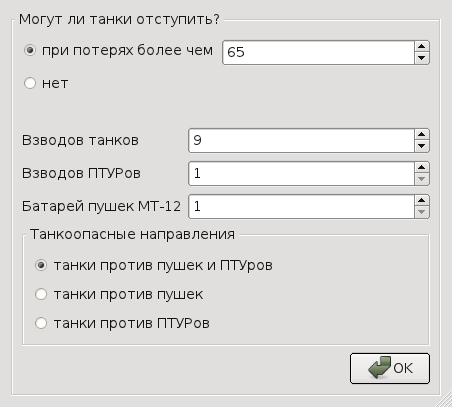
\includegraphics[height=70mm]{img1.png}
\end{center}
Присутствуют следующие настройки модели боя.
\begin{itemize}
 \item Танки отступят при потере указанного (в процентах) количества личного состава.
 \item Танки не отсупают.
 \item Количество взводов танков: от 1 до трех, по 18 танков во взводе.
 \item Количество подразделений ПТУРов.
 \item Количество подразделений гаубиц Д-30.
 \item Танкоопасные направления
   \begin{itemize}
    \item Танки против ПТУРов и гаубиц
    \item Танки против гаубиц
    \item Танки против ПТУРов
   \end{itemize}
\end{itemize}


\section{Моделирование}

\end{document}
